\section{Introduction}
Electrokinetic theory describes the dynamics of charged particles
in ionic fluids \cite{kirby2010book}. When a particle acquires surface charge, a layer
of ions of opposite charge is attracted to the surface via
electric forces, creating a double-layer structure around the
particle (see Figure \ref{fig:EDL}). This structure, called
``Debye layer'', electrically screens the surface charge, thus
creating a potential difference between the particle and the outer
layer of the fluid bulk.
\begin{figure}[htbp]
\begin{framed}
    \begin{center}
        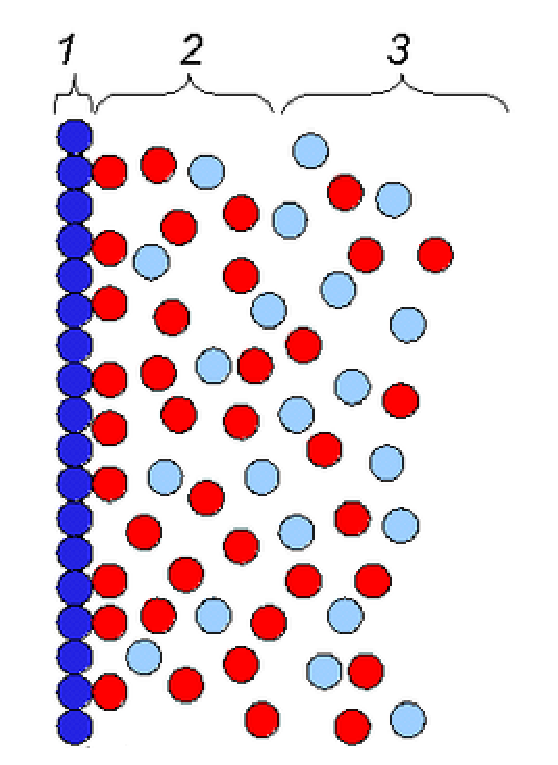
\includegraphics[width=0.25\textwidth]
            {figs/ElectricDoubleLayer.eps}
        \caption{Schematic structure of the double layer:
        (1) particle surface, (2) Debye layer and (3) fluid bulk.
        If the particle surface has positive (blue) surface charge,
        it attracts negative (red) ions from the fluid making the
        Debye layer negatively charged (as opposed to the rest of
        the fluid bulk, which is electrically neutral).
        The zeta potential is defined as the voltage drop across (2).}
        \label{fig:EDL}
    \end{center}
\end{framed}
\end{figure}
In cases where the layer width is much smaller than the particle's
size, an analytical asymptotic solution for the Debye layer
dynamics can be found \cite{yariv2010asymptotic}.

The partial differential equations that descibe the system dynamics
are coupled and non-linear. 
In general, they have no analytic solution. Moreover,
any numerical solver must handle the scale disparity caused by the
Debye layer width being much smaller than the particle's size. A
closed-form linear asymptotic solution has been developed for
spherical particles and weak electric field in an
axisymmetric setting \cite{yariv2010migration, schnitzer2012surface} but it is hard to extend this
analytic solution to more general systems. Once the electric field
becomes stronger, significant nonlinear phenomena are expected.
This interesting regime has not yet been explored.

Recently, it has been conceived that such type of dynamics
can be very useful in transporting and manipulating micro-
and nanoscale objects for many nanotechnology applications,
such as the self-assembly of superstructures, roving sensors, 
drug-delivery systems and useful nanomachinery 
\cite{howse2007self,paxton2004catalytic,pumera2010electrochemically}.
However, since the analytic model for these electrokinetic
phenomena has no closed-form analytic solution, a numerical
solver has to be developed for analysing such system.



%%%%%%%%%%%%%%%%%%%%%%%%%%%%%%%%%%%%%%%%%%%%%%%%%%%%%%%%%%%%%%%%%%%%%%%%%%%%%%%%%%%%%%%%%%%%%%%%%%
\subsection{Micro-scale phenomena}

\subsubsection{Dimensionless Notation}

Spatial coordinates $\br$ are normalized by $a^*$ (the characteristic size of the particle).

Positive and negative ionic concentrations are denoted by $c_+$ and $c_-$ respectively, and
are normalized by ambient ionic concentration $c^*$. The ionic valences are $\pm z$.

The dimensional ionic fluxes are given by Nernst-Plank equation 
(using Einstein relation for the electric mobility, $\mu_q^* = D^* / k_B^* T^*$):
\begin{eqnarray}
\bj^*_\pm &=& 
-D^* \bnabla c^*_\pm + \bv^* c^*_\pm \mp \frac{z e^* D^*}{k_B^* T^*} c^*_\pm \bnabla \varphi^*,
\end{eqnarray}
where $D^*$ is the ionic diffusivity.

The electric potential $\varphi$ is normalized by the thermal voltage:
\begin{eqnarray}
\varphi^* &=& \frac{k_B^* T^*}{z e^*} = \frac{R^* T^*}{z F^*},
\end{eqnarray}
where $R^* = k_B^* N_A$ and $F^* = e^* N_A$ is the Faraday number.

The dimensional Stokes equation:
\begin{eqnarray}
-\bnabla p^* + \mu^* \bLaplacian \bv^* + \eps^* \Laplacian \varphi^* \bnabla \varphi^* &=& 0.
\end{eqnarray}

The velocity $\bv$ is normalized by:
\begin{eqnarray}
v^* &=& \frac{\eps^* (\varphi^*)^2}{a^* \mu^*},
\end{eqnarray}
and the pressure $p$ is normalized by:
\begin{eqnarray}
p^* &=& \frac{\mu^* v^*}{a^*} = \frac{\eps^* (\varphi^*)^2}{(a^*)^2}.
\end{eqnarray}

The fluxes $\bj^*_\pm$ are normalized by:
\begin{eqnarray}
j^* = \frac{D^* c^*}{a^*}.
\end{eqnarray}

The nondimensional Nernst-Plank equation is written as:
\begin{eqnarray}
\bj_\pm &=& 
-\bnabla c_\pm + \alpha \bv c_\pm \mp c_\pm \bnabla \varphi, \\
\alpha &=&
\frac{v^* a^*}{D^*} = \frac{\eps^* (\varphi^*)^2}{\mu^* D^*}.
\end{eqnarray}
where $\alpha$ is the dimensionless Peclet number.

The dimensional Poisson equation is:
\begin{eqnarray}
(c^*_+ - c^*_-) z e^* &=& -\eps^* \Laplacian \varphi^*,
\end{eqnarray}
and after nondimensionalization, is:
\begin{eqnarray}
c_+ - c_- &=& -\frac{\eps^* \varphi^*}{z e^* c^* (a^*)^2} \Laplacian \varphi = 
-2\delta^2 \Laplacian \varphi,
\\
\delta^2 &=& \frac{\eps^* \varphi^*}{2c^* e^* z (a^*)^2} = 
\pars{\frac{\delta^*}{a^*}}^2.
\end{eqnarray}

The force is denoted by $\bF$ normalized by $\mu^* v^* a^* = \eps^* (\varphi^*)^2$.
The stress tensor is denoted by $\tT$ and normalized by $p^* = \mu^* v^* / a^*$.
The electric field is denoted by $\bE$ and normalized by $E^* = \varphi^* / a^*$.

\subsubsection{Nernst-Planck Equations}
The ionic fluxes are given by ion diffusion, electrostatic forces and ion advection by the fluid:
\begin{eqnarray}
  \bj_\pm &=& -\bnabla c_\pm \mp c_\pm \bnabla \varphi + \alpha \bv c_\pm,
\end{eqnarray}

Due to conservation of ions, the fluxes are divergence-free:
\begin{eqnarray}
\bnabla \cdot \bj_\pm &=& 0.
\end{eqnarray}
These equation may be re-written by using the following transform:
\begin{eqnarray}
  c &=& \frac{c_+ + c_-}{2},\\
  q &=& \frac{c_+ - c_-}{2}.
\end{eqnarray}
Thus, salt and charge fluxes are defined by:
\begin{eqnarray}
  \bj &=& \frac{\bj_+ + \bj_-}{2} = -\bnabla c - q \bnabla \varphi + \alpha \bv c, \\
  \bi &=& \frac{\bj_+ - \bj_-}{2} = -\bnabla q - c \bnabla \varphi + \alpha \bv q,
\end{eqnarray}
and are divergence-free as well:
\begin{eqnarray}
\bnabla \cdot \bj &=& 0, \\
\bnabla \cdot \bi &=& 0. 
\end{eqnarray}

\subsubsection{Incompressible Stokes Flow with Electrostatic Force}
Mass conservation (due to constant fluid density):
\begin{eqnarray}
\bnabla \cdot \bv &=& 0.
\end{eqnarray}
Momentum conservation (force balance):
\begin{eqnarray}
\Laplacian \bv - \bnabla p + \bnabla \varphi \Laplacian \varphi &=& 0.
\end{eqnarray}
Free charge density is given by the Poisson equation:
\begin{eqnarray}
\delta^2 \Laplacian \varphi &=& -q.
\end{eqnarray}

\subsubsection{Boundary conditions}
An constant electric field $\bE$ is applied to the system, such that $|\bE| = \beta$.
The particle will acquire a non-zero steady-state velocity $\cU$, which is
a function of the applied field, and is not known a priori.

Far away from the particle, we have uniform applied electrostatic field, uniform flow 
and ambient ionic concentrations:
\begin{eqnarray}
\bv &\rightarrow& -\cU \ui, \\
\bE = -\bnabla \varphi &\rightarrow& \beta\ui, \\
c_\pm &\rightarrow& 1.
\end{eqnarray}

We consider a spherical particle. 
At its surface $\mathcal{S}$ (defined at $r=1$ with normal $\bn = \brhat$), 
we have zero slip and ion impermeability.
\begin{eqnarray}
\bv & = & \bzero, \\
\bn \cdot \bj_\pm & = & 0.
\end{eqnarray}

%%%%%%%%%%%%%%%%%%%%%%%%%%%%%%%%%%%%%%%%%%%%%%%%%%%%%%%%%%%%%%%%%%%%%%%%%%%%%%%%%%%%%%%%%%%%%%%%%%
\subsection{Bulk-scale equations}
When $\delta \ll 1$, 
most of the fluid remains electroneutral ($q \approx 0$, thus $c_+ \approx c_-$), 
except a thin boundary layer of width $O(\delta)$, 
also known as the ``Debye layer'', surrounding the ion exchanger. 

The Nernst-Planck equations above for the fluid bulk (outside
the boundary layer), using bulk variables, read:
\begin{eqnarray}
  Q & = & 0, \\
  C & = & C_+ = C_-, \\
\bJ &=& -\bnabla C + \alpha \bV C, \\
\bI &=& -C \bnabla \varPhi.
\end{eqnarray}
Because the flow is incompressible ($\bnabla \cdot V = 0$), 
ion conservation results in the following equations:

\begin{enumerate}
\item Salt conservation macroscale equation:
\begin{eqnarray}
\bnabla \cdot \bJ = \Laplacian C - \alpha \bV \cdot \bnabla C = 0. 
\end{eqnarray}

\item Charge conservation macroscale equation:
\begin{eqnarray}
\bnabla \cdot \bI = \bnabla \cdot \pars{ C \bnabla \varPhi } = 0.
\end{eqnarray}
\end{enumerate}

The macroscale Stokes flow equations have the same form as the microscale equations:
\begin{eqnarray}
\bnabla \cdot \bV &=& 0, \\
\Laplacian \bV - \bnabla P + \bnabla \varPhi \Laplacian \varPhi &=& 0.
\end{eqnarray}

\subsection{Debye-scale effective boundary conditions}
The effective boundary conditions depend on the specific physical and chemical properties 
of the particle. We consider the following scenarios:

\subsubsection{Inert particle}

We define the scaled coordinate $\rho$ (normal to ion-exchanger surface), where $\delta \ll 1$:
\begin{eqnarray}
  \rho &=& \frac{r-1}{\delta}. 
\end{eqnarray}
Thus, the electric potential and the ionic concentrations are $O(1)$ at the Debye layer ($r \approx 1$):
\begin{eqnarray}
  \varphi(\rho,\theta) &\sim& \varphi, \\
  c_\pm(\rho,\theta) &\sim& c_\pm, \\
  c(\rho,\theta) &\sim& c, \\
  q(\rho,\theta) &\sim& q.
\end{eqnarray}

The radial fluxes at the Debye layer are $O(\delta^{-1})$, due to coordinate rescaling:
\begin{eqnarray}
  j_\pm(\rho, \theta) &\sim& \delta^{-1} j_\pm.
\end{eqnarray}

The pressure is $O(\delta^{-2})$, due to momentum balance equations:
\begin{eqnarray}
  p(\rho, \theta) &\sim& \delta^{-2} p.
\end{eqnarray}

The tangential velocity component is $O(1)$ and the radial component is $O(\delta)$.

In order to match bulk $O(1)$ outer radial ionic flux, 
the $O(\delta^{-1})$ term of the inner ionic radial flux, $j_\pm(\rho, \theta)$ must vanish:
\begin{eqnarray}
  -\deriv{c_\pm}{\rho} \mp c_\pm \deriv{\varphi}{\rho} &=& 0, \\
  \deriv{\varphi}{\rho} \pm\frac{1}{c_\pm}\deriv{c_\pm}{\rho} &=& 0, \\
  \pars{\varPhi - \varphi} \pm\pars{\log C_\pm - \log c_\pm} &=& 0, \\
  \varPhi - \varphi \pm \log \frac{C_\pm}{c_\pm} &=& 0.
\end{eqnarray}
This relation can be rewritten as a Boltzmann distribution of ionic concentration:
\begin{eqnarray}
\lim_{\rho\rightarrow\infty} c_\pm &=& C, \\
c_\pm &=& C \exp\left[\pm(\varPhi - \varphi)\right].
\end{eqnarray}

Due to ion impermeability and radial flux continuity:
\begin{eqnarray}
  \br \cdot \bj_\pm = -\deriv{c_\pm}{r} \mp c_\pm \deriv{\varPhi}{r} &=& 0, \\
-\deriv{C}{r} \mp C \deriv{\varPhi}{r} &=& 0, \\
\deriv{C}{r} = \deriv{\varPhi}{r} &=& 0.
\end{eqnarray}

Using the derivation in Appendix \ref{append:slip} and the fact that $V_r = 0$ 
on the boundary, the slip condition can be written using the surface
gradient operator:
\begin{eqnarray}
\bV &=& 
\zeta \cdot \bnabla_\mathcal{S} \varPhi 
+ 2\log\pars{1-\tanh^2\frac{\zeta}{4}} \cdot \bnabla_\mathcal{S} \log C, \\
\bnabla_\mathcal{S} &=& \pars{\tI - \bn\bn} \bnabla.
\end{eqnarray}

\subsubsection{Ion-exchanger}

Due to cation selectivity, $c_+|_{\rho=0} = \gamma$.
\begin{eqnarray}
  c_+ = \gamma &=& C \exp(\varPhi - \cV), \\
  \cV + \log \gamma &=& \log C + \varPhi.
\end{eqnarray}

The so-called zeta potential is 
the voltage drop between the particle surface and the end of
the boundary layer, denoted $\zeta = \cV - \varPhi$. 

Without loss of generality, 
we assume that $\cV = -\log\gamma$, thus $\zeta = -\log\gamma-\varPhi$:
\begin{eqnarray}
\varPhi + \log C &=& 0.
\end{eqnarray}

Due to anion impermeability and radial flux continuity:
\begin{eqnarray}
  \br \cdot \bj_- = -\deriv{c_-}{r} + c_- \deriv{\varPhi}{r} &=& 0, \\
-\deriv{C}{r} + C \deriv{\varPhi}{r} &=& 0, \\
\deriv{}{r}\pars{\varPhi - \log C} &=& 0.
\end{eqnarray}

\subsubsection{Highly charged particle}
\begin{eqnarray}
 \deriv{C}{r} + C \deriv{\varPhi}{r} &=& 0, \\
 \deriv{C}{r} - \mbox{Du} \Laplacian_s (\varPhi - \log C) &=& 0.
\end{eqnarray}


\subsection{Steady state}
The stress tensor is composed of Newtonian and Maxwel stresses:
\begin{eqnarray}
\tT &=& \bnabla \bV + (\bnabla \bV)^\dagger - P \tI
+ \bnabla \varPhi \bnabla \varPhi - \frac{1}{2} (\bnabla \varPhi \cdot \bnabla \varPhi) \tI, \\
\bnabla \cdot \tT &=& \bzero.
\end{eqnarray}
The total force acting on the particle is computed by the following surface integral:
\begin{eqnarray}
\bF &=& \oint_\mathcal{S} \tT \cdot \bnhat dA.
\end{eqnarray}
In steady state (constant particle drift velocity $\cU$), 
the total force must be zero: 
\begin{eqnarray}
\bF = \bzero.
\end{eqnarray}

The total force $\bF(\beta, \cU)$ is a function of the applied electric field $\beta$ and
the velocity $\cU$.
For any given electric field $\beta$, the force-free constraint above 
can be solved numerically for $\cU$ to
yield the corresponding steady-state velocity.
